\section{Analysen af problemet}

For at give en grundlægge specifikation til systemet, skal problemet op udspecificeres.  

Graf \ref{vandspild_graf_normal} viser et eksempel på hvordan temperaturændringerne forekommer, hvis det antages at vandspildet negliseres og temperaturen på røret derfor er lig med temperaturen i rummet. 
\\
\\
\begin{figure}[h!]
  \centering
  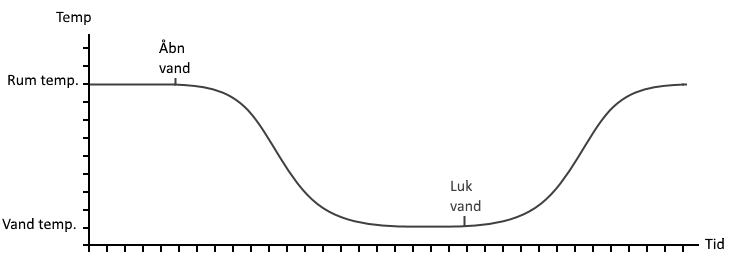
\includegraphics[width=0.7\textwidth]{figures/vandspild_graf_normal.png}
  \caption{Grafen viser overvågningssystemet uden vand spild.}
  \label{vandspild_graf_normal}
\end{figure}
\\
\\
Tilførelsen af nyt vand til huset ændre rørets temperatur og derfor vil der forekomme temperatursvingninger, som målingen viser vandspildet ud fra. Nedernstående graf \ref{vandspild_graf_spild} viser et eksempel på temperaturændringer ved vandspild på et rør.
\\
\\
\begin{figure}[h!]
  \centering
  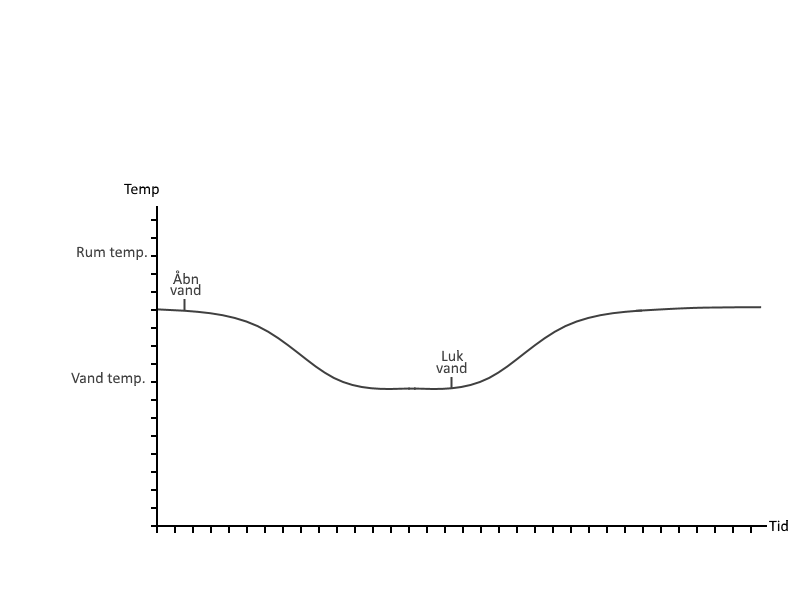
\includegraphics[width=0.7\textwidth]{figures/vandspild_graf_spild.png}
  \caption{Grafen viser overvågningssystemet med vandspild.}
  \label{vandspild_graf_spild}
\end{figure}
\\
\\
På graf \ref{vandspild_graf_spild} ses det hvordan hviletemperaturen på røret aldrig når temperaturen i rummet, da vandet aldrig ligger helt stille og derfor tilfører en konstant koldere temperatur.
\\
\\
Ud fra graferne \ref{vandspild_graf_normal} og \ref{vandspild_graf_spild}, ses forskellen tydeligt og det kan konkluderes at der er et problem, som i denne rapport ikke skal løses med en funktionel regulærbar løsning, men med måleender som skal give kunden et overblik over omfanget af spildevand.
\\
\\
Produktet skal kunne overvåge vandspildet uden at have regulerbare funktioner. Det skal kunne måle temperaturen i henholdvis rummet og overfladen på vandrøret, endvidere skal det kunne sammenligne de to temperature.
\\
\\
Kravene for produktet er opstillet i det efterfølgende afsnit.     